\newpage

\subsection{Fonony w materiale}
\textbf{Fonon} jest kwazicząstką (bozonem), lub inaczej kwantem energii drgań sieci krystalicznej. Wyróżnia się dwa rodzaje fononów:
\begin{itemize}
	\item{Fonony akustyczne. Rozchodzą się w sieci krystalicznej, gdy mamy do czynienia z jednym atomem w komórce elementarnej.}
	\item{Fonony optyczne. Pojawiają się w sieci krystalicznej oprócz fononów akustycznych gdy mamy więcej niż jeden atom w komórce elementarnej.}
\end{itemize}
Podział fononów jest uzależniony od kształtu relacji dyspersji w pobliżu k=0. \\
Fonony akustyczne wykazują zależność:
\begin{equation}
	\lim_{k \to 0} \omega(k) = 0
\end{equation}
natomiast fonony optyczne:
\begin{equation}
\lim_{k \to 0} \omega(k) = const
\end{equation}
\begin{figure}[H]
	\begin{center}
		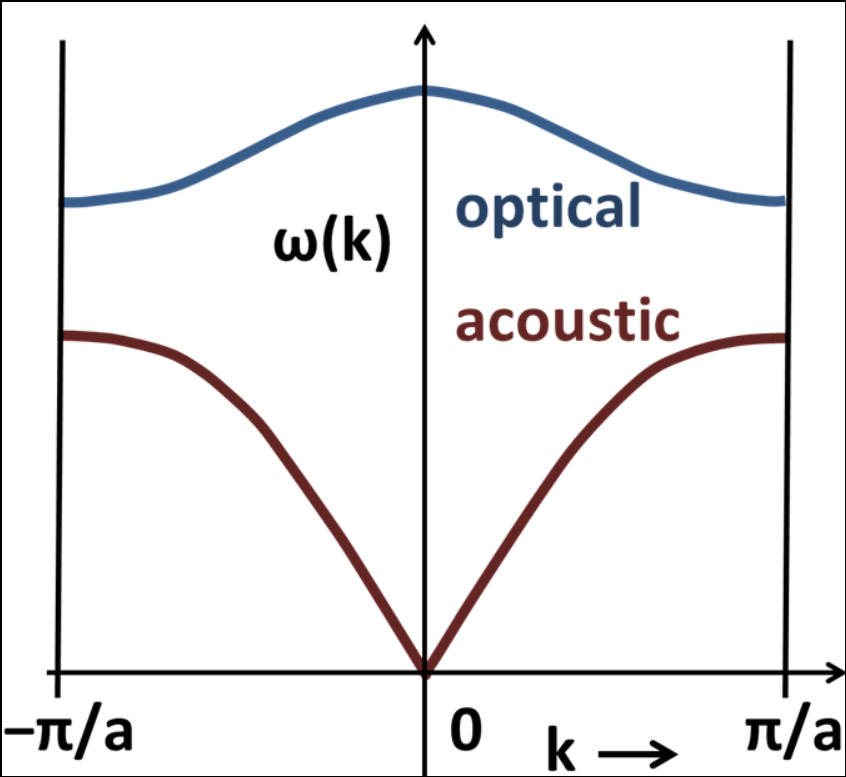
\includegraphics[width=0.6\linewidth]{Rozpraszanie-Ramanowskie-Ciekie/Phonons.png}
		\caption{Krzywe dyspersji dla liniowego łańcucha dwuatomowego.}
	\end{center}
\end{figure}
Dla kryształu zawierającego N(>1) różnych atomów w komórce elementarnej relacja dyspersji zawiera $\alpha$ gałęzie akustycznych oraz $\alpha$N-$\alpha$ gałęzi optycznych, gdzie $\alpha$ jest wymiarem kryształu. Wobec tego dla liniowego łańcucha dwuatomowego N=2 mamy jedną gałąź optyczną i jedną akustyczną, a dla trójwymiarowej komórki prostej zawierającej dwa różne atomy będziemy mieli 3 gałęzie optyczne i akustyczne.

Przy rozpraszaniu fotonów na fononach są spełnione dwa prawa zachowania: 

Prawo zachowania energii:
\begin{equation}
	\hbar \mathbf{\omega_{i}} = \hbar \mathbf{\omega_{s}} \pm \hbar \mathbf{\Omega_{fonon}}
\end{equation}
\begin{itemize}
	\item $\omega_{i}$ - częstotliwość fotonu padającego;
	\item $\omega_{s}$ - częstotliwość fotonu rozproszonego;
	\item $\Omega_{fonon}$ - częstotliwość fononu;
	\item $\hbar$ - stała Plancka zredukowana.
\end{itemize}

Prawo zachowania pędu:
\begin{equation}
	\hbar \mathbf{k_{i}} = \hbar \mathbf{k_{s}} \pm \hbar \mathbf{K_{fonon}}
\end{equation}
\begin{itemize}	
	\item $k_{i}$ - wektor falowy fotonu padającego;
	\item $k_{s}$ - wektor falowy fotonu rozproszonego;
	\item $K_{fonon}$ - wektor falowy fononu;
\end{itemize}

Pęd fononu jest znacznie większy od pędu fotonu, a energia fotonu jest 
znacznie większa od energii fononu. To oznacza że w oddziaływaniu uczestniczą fonony o małym pędzie.

\begin{figure}[H]
	\begin{center}
		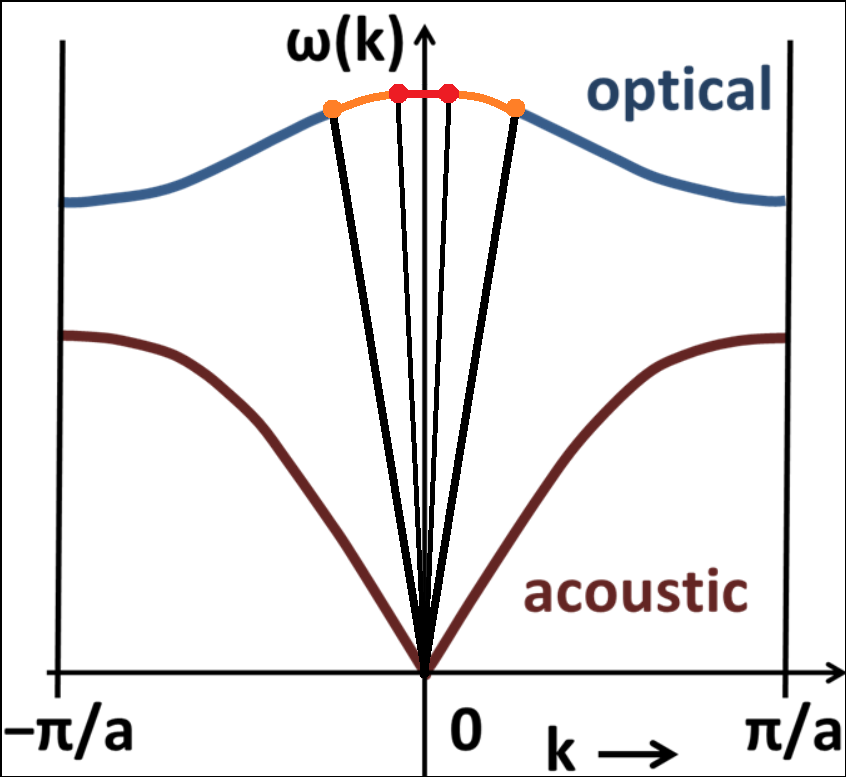
\includegraphics[width=0.6\linewidth]{Rozpraszanie-Ramanowskie-Ciekie/PhononsCenter.png}
		\caption{Krzywe dyspersji z zaznaczonym obszarem, pokazującym które fonony uczestniczą w rozpraszaniu ramanowskim.}
	\end{center}
\end{figure}

Z powyższego rysunku widzimy, że w oddziaływaniach biorą udział tylko  fonony optyczne zlokalizowane w środku strefy Brillouina. oddziaływanie fononów akustycznych z fotonami możemy zaniedbać dlatego, że dla $k \rightarrow 0$ energia fononów akustycznych też dąży do zera.

W niniejszej pracy były badane tylko widma stokesowskie które są dużo bardziej intensywne niż widma antystokesowskie. Miarą intensywności widma są piki, które uzyskujemy. Im większe natężenie danego piku, tym mniejszy błąd popełniamy przy analizie wyników pomiaru.
Prawdopodobieństwo obsadzenia stanu energetycznego fononem jest proporcjonalne do:
\begin{equation}
	\sim \exp^{-\frac{E}{kT}} 
\end{equation}
\begin{itemize}
	\item{$E$ - energia stanu energicznego};
	\item{$k$ - stała Boltzmanna};
	\item{$T$ - temperatura w Kelwinach}.
\end{itemize}
To oznacza że stosunek intensywności promieniowania rozproszonego w widmie antystokesowskim do intensywności promieniowania stokesowskiego jest:
\begin{equation}
	\frac{I_{ants}}{I_s} \sim \exp^{-\frac{E}{kT}}
\end{equation}
\begin{itemize}
	\item{$I_{ants}$ - intensywność promieniowania w widmie antystokesowskim};
	\item{$I_s$ - intensywność promieniowania w widmie stokesowskim}
\end{itemize}
	Dla energii fononu $E = 0.065eV$:
\begin{equation}
	\sim \exp^{-\frac{E}{kT}} = \exp^{-\frac{0.065}{0.025}} \approx 0.07
\end{equation}
Czyli intensywność widma antystokesowskiego wynosi $7\%$ w stosunku do widma stokesowskiego. 
\subsection{Co można odczytać z widma ramanowskiego?}
Ważną rolę w widmie ramanowskim odgrywa szerokość połówkowa pików.
Na podstawie informacji o szerokości połówkowej $\Gamma$ można mówić o czasie życia fononów w próbce:
\begin{equation}
	\Gamma \sim \frac{1}{\tau}
\end{equation}

gdzie $\tau$ - czas życia fononu.

\begin{figure}[H]
	\begin{center}
		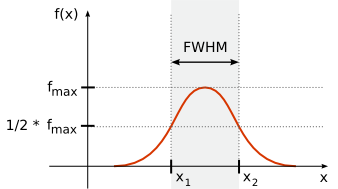
\includegraphics[width=0.8\linewidth]{Full_width_at_half_maximum.png}
		\caption{Szerokość połówkowa piku \textit{FWHM} - z angielskiego \textit{Full Width at Half Maximum}.}
	\end{center}
\end{figure}

Szerokość połówkowa zależy od:
\begin{itemize}
	\item[1]{Rozmiaru próbki -- czy materiał jest 0,1,2 czy 3 wymiarowy.}
	\item[2]{Defektów i niedoskonałości sieci krystalicznej. Fonony rozpraszają się na defektach, co zmniejsza czas ich życia.}
	\item[3]{Rozpraszanie fononów wskutek efektów anharmonicznych.}
\end{itemize}
Na podstawie zmian szerokości pików w funkcji temperatury można uzyskać informacje o przewodnictwie cieplnym próbki. 
W zależności od liczby i kształtu pików ramanowskich można określić rodzaj materiału, oraz jakość krystaliczną materiału.
Na podstawie widma Ramanowskiego można również oszacować temperaturę próbki. Czyli jest możliwy bezkontaktowy pomiar temperatury na podstawie widma ramanowskiego.

\subsection{Piki ramanowskie w cienkich warstwach}
W materiałach cienkowarstwowych jeden z wymiarów jest rzędu kilku nanometrów. To powoduje że zaczynają odgrywać ważną rolę efekty kwantowe. Z zasady nieoznaczoności Heisenberga:
\begin{equation}
	\Delta p_{fon} \Delta d \geq \frac{\hbar}{2}
\end{equation}
\begin{itemize}
	\item{$\Delta p_{fon}$ - niepewność pomiaru pędu fononu};
	\item{$\Delta d$ - rozmiar obszaru w którym rozchodzi się fonon}
\end{itemize}
Ograniczenie rozmiaru obszaru w którym rozchodzi się fonon skutkuje większą niepewnością określenia pędu fononu, a stąd również wektora falowego fononu. To znaczy że w rozpraszaniu ramanowskim będą uczestniczyć optyczne fonony o  energiach z przedziału, wyznaczonego przez krzywą dyspersji dla tego fononu. Przykładowo fonony biorące udział w oddziaływaniu z fotonami zaznaczone są kolorem czerwonym bądź pomarańczowym w obszarze pierwszej strefy Brillouine'a na poniższym rysunku.

\begin{figure}[H]
	\begin{center}
		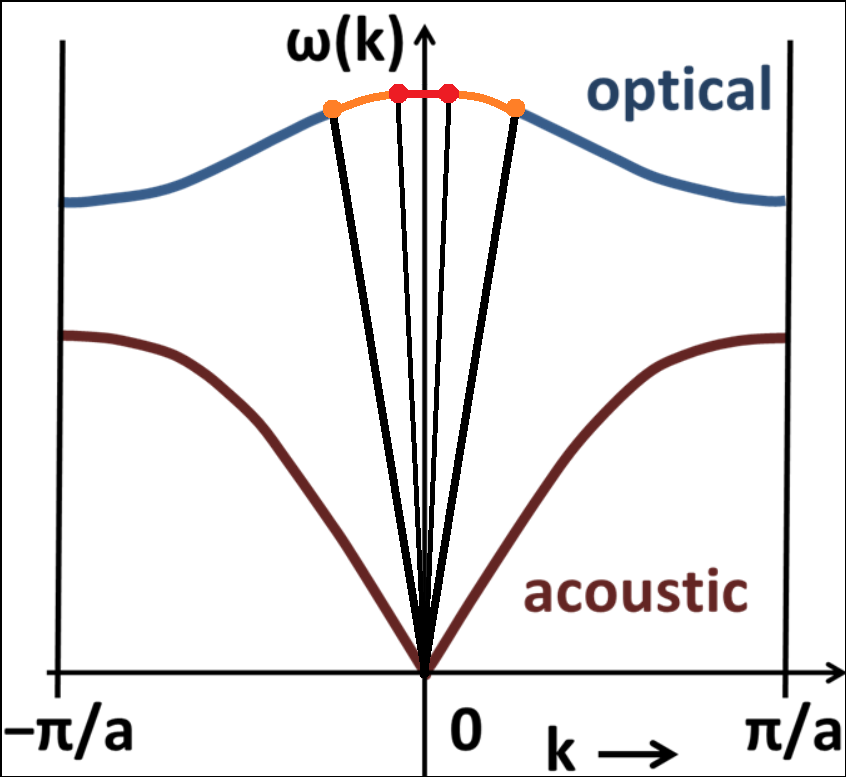
\includegraphics[width=0.6\linewidth]{Rozpraszanie-Ramanowskie-Ciekie/PhononsCenterQuantum.png}
		\caption{Krzywe dyspersji z zaznaczonym obszarem, pokazującym, które fonony uczestniczą w rozpraszaniu ramanowskim w cienkich warstwach.}
	\end{center}
\end{figure}

Taka rozbieżność w energii wpływa na kształt powstających pików w widmie ramanowskim.Piki te są z reguły poszerzone oraz przesunięte w kierunku mniejszych energii (red-shift). Widoczna również asymetria w kształcie pików, jak jest pokazane na poniższym rysunku:

\begin{figure}[H]
	\begin{center}
		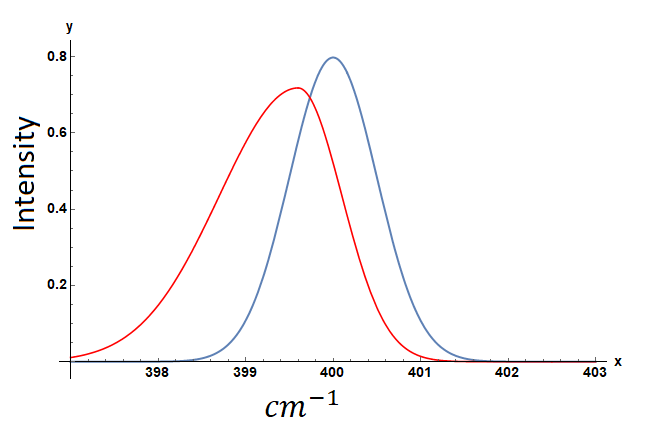
\includegraphics[width=0.7\linewidth]{Rozpraszanie-Ramanowskie-Ciekie/piki.png}
		\caption{Pik ramanowski dla próbek objętościowych(Niebieski), oraz przykładowy pik ramanowski w cienkich warstwach(Czerwony)}
	\end{center}
\end{figure}

Spotyka się również krzywe dyspersji fononu, gdzie energia fononu jest mniejsza w środku strefy Brillouine'a niż w innych punktach tej strefy. Wtedy zjawisko "Phonon confinement" będzie skutkowało przesunięciem piku w stronę wyższych energii (Blue-shift).

\subsection{Rozpraszanie dwufononowe}
Kiedy foton trafia na próbkę może zajść sytuacja, że w materia zostaną wykreowane dwa fonony o przeciwnych pędach prawie takich samych co do wartości. Wtedy również będzie spełniona zasada zachowania pędu. Takie przykładowe dwa fonony zostały przedstawione na rysunku niżej. Fonony te nie muszą należeć do tej samej krzywej dyspersji. 
 
\begin{figure}[H]
	\begin{center}
		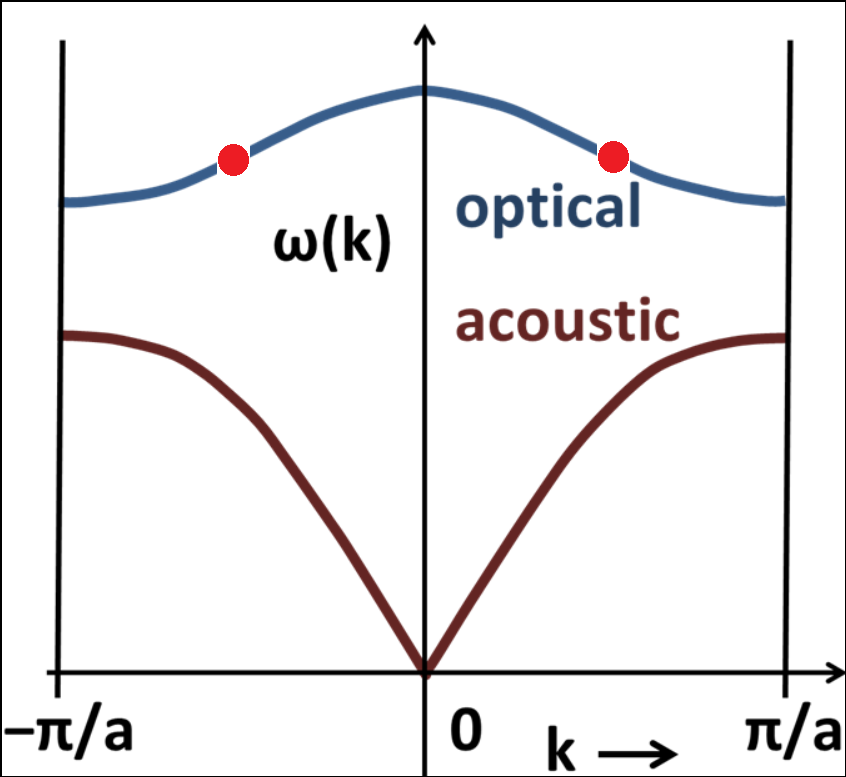
\includegraphics[width=0.55\linewidth]{Rozpraszanie-Ramanowskie-Ciekie/Phonons_opposite.png}
		\caption{Przykład wykreowania dwóch fononów o przeciwnych wektorach falowych przy jednoczesnym spełnieniu zasady zachowania pędu ($k \sim 0$).}
	\end{center}
\end{figure}

Piki na widmie ramanowskim pochodzące z rozpraszania dwufononowego mają prawie dwa razy większą energię (częstotliwość) niż piki jednofononowe ze środka strefy Brillouine'a.

\subsection{Widmo ramanowskie w funkcji polaryzacji}

W zależności od kierunku polaryzacji światła laserowego padającego, oraz polaryzacji światła rozproszonego ramanowsko intensywności pików będą się zmieniać. Po zarejestrowaniu zmian natężenia piku ramanowskiego w funkcji kąta polaryzacji można uzyskać ramanowskie widmo polaryzacyjne. Przykładowe widmo polaryzacyjne dla różnych modów drgań (fononów) jest przedstawiono poniżej:

\begin{figure}[H]
	\begin{center}
		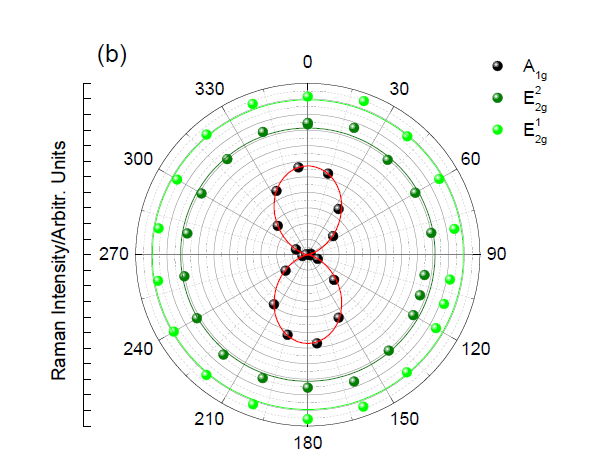
\includegraphics[width=0.8\linewidth]{Wlasciwosci/Spectre-polarization-Ga2S3.png}
		\caption{Przykładowe widmo polaryzacyjne dla trzech modów drgań $\mathbf{A_{1g}}$ $\mathbf{E_{2g}^{2}}$ $\mathbf{E_{2g}^{1}}$ w $\mathbf{MoTe_{2}}$. Natężenie piku (pole powierzchni ograniczone pikiem) przedstawione zostało jako odległość od środka wykresu. Jest to tak zwany wykres Arrheniusa. Kąt występujący w pomiarach polaryzacyjnych jest zawarty pomiędzy kierunkiem polaryzacji promieniowania pobudzającego a wyróżnionym kierunkiem w przestrzeni. Na rysunku widać, że tylko pik $\mathbf{A_{1g}}$ znacząco reaguje na zmianę kąta polaryzacji [19].}
	\end{center}
\end{figure}

Intensywność piku ramanowskiego można przedstawić w postaci:
\begin{equation}
I_{s} \sim |e_{s}\mathbf{R}e_{i}|^{2}
\end{equation}
Gdzie,
\begin{itemize}
	\item $e_{i}$ i $e_{s}$ - wektory polaryzacji promieniowania podającego i rozproszonego odpowiednio.
	\item $\mathbf{R}$ - tensor ramanowski, który zależy od symetrii kryształu i rodzaju drgającego modu.
\end{itemize}

Wektor polaryzacji rozproszonego światła ramanowskiego jest powiązany z wektorem polaryzacji światła padającego przez charakterystyczny tensor ramanowski. Unikalny tensor ramanowski istnieje dla każdego aktywnego
modu ramanowskiego.

Tensor ramanowski jest macierzą 3 x 3, i w przypadku cząsteczek chemicznych (molekuł) łączy wyindukowany moment dipolowy ($x_{2}$, $y_{2}$, $z_{2}$) z wektorem natężenia pola elektrycznego ($x_{1}$, $y_{1}$, $z_{1}$).

\begin{figure}[H]
	\begin{center}
		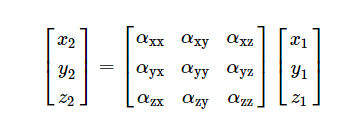
\includegraphics[width=0.5\linewidth]{Wlasciwosci/Raman-Tensor.png}
	\end{center}
\end{figure}

Tensor ramanowski jest tensorem symetrycznym: $a_{xy} = a_{yx}$, $a_{yz} = a_{zy}$, $a_{zx} = a_{xz}$, wobec tego ma co najwyżej 6 różnych składowych. W tym przypadku x, y i z są osiami układu kartezjańskiego. Istnieją standardowe metody wyboru kierunku tych osi w zależności od symetrii układu. Jeśli jako osie układu przyjmiemy główne osie tensora ramanowskiego, to sześć niezerowych współczynników tensora redukuje się do trzech elementów diagonalnych: $a_{xx}$, $a_{yy}$ i $a_{zz}$. W takim przypadku tensor Ramana może zostać wyznaczony przez podanie $a_{xx}$, $a_{yy}$ i $a_{zz}$ oraz trzech parametrów kątowych, które ustalają orientacje głównych osi tensora w układzie współrzędnych $xyz$.

Przykładowo, aby zdefiniować system głównych osi lokalnego tensora ramanowskiego, arbitralnie wybieramy trzy nieliniowo ułożone atomy $E_1$, $E_2$ i $A$ w cząsteczce będącej przedmiotem zainteresowania w taki sposób, że oś $y$ jest równoległa do linii łączącej atomy $E_1$ i $E_2$, zaś oś $x$ jest równoległa do linii prostopadłej łączącej atom $A$ z osią $y$, a oś $z$ jest prostopadła do osi $y$ i $x$. Chociaż zestaw wybranych osi może nie obejmować całego kąta bryłowego 4$\pi$, zwykle wystarcza do określenia tensora Ramana. Wynika to z faktu, że każda przerwa między kierunkami dwóch kandydujących osi wprowadza błąd, który jest mały w stosunku do błędów w pomiarach eksperymentalnych.
